%!TEX encoding = UTF-8 Unicode

%!TEX root = ../compendium.tex

\Lab{\LabWeekSIX}

\begin{Goals}
\item Kunna skapa egna klasser.
\item Förstå skillnaden mellan klasser och objekt.
\item Förstå skillnaden mellan muterbara och omuterbara objekt.
\item Förstå hur ett objekt kan innehålla referenser till objekt av andra klasser, och varför detta kan vara användbart.
\item Träna på att fatta beslut om vilka datatyper som bäst passar en viss tillämpning.
\end{Goals}

\begin{Preparations}
\item \DoExercise{\ExeWeekSIX}{06}


\end{Preparations}

\subsection{Bakgrund}

Under den här laborationen ska du skriva en samling av klasser som tillsammans kan användas för att rita i en fönsterruta. För att ge dig en grund att stå på får du tillgång till den färdigskrivna klassen SimpleWindow. SimpleWindow är en fönsterruta som tillåter programmeraren att rita linjer med hjälp utav en  ''penna''. SimpleWindow håller koll på pennans nuvarande position och kan ombes att flytta pennan genom att antingen lyfta den eller genom att rita en rak linje till en ny position.

\begin{JavaSpec}{class SimpleWindow}
  /** mouse click event type */
	public final static int MOUSE\_EVENT = 1;

  /** key pressed event type */
	public final static int KEY\_EVENT = 2;

  /** window closed event type */
	public final static int CLOSE\_EVENT = 3;

  /** Creates a window and makes it visible. */
	public SimpleWindow(int width, int height, String title);

  /** Returns the width of the window. */
	public int getWidth();

	/** Returns the height of the window. */
	public int getHeight();

	/** Clears the window. */
	public void clear();

	/** Closes the window.*/
	public void close();

	/** Opens the window. */
	public void open(); 

	/** Moves the pen to a new position. */
	public void moveTo(int x, int y) ;

	/** Moves the pen to a new position while drawing a line. */
	public void lineTo(int x, int y);

	/** Writes a string at the current position.* /
	public void writeText(String txt);
	
	/** Draws a bitmap image at the current position.*/
	public void drawImage(Image image);

	/** Returns the pen's x coordinate. */
	public int getX();

	/** Returns the pen's y coordinate. */
	public int getY();

	/** Sets the line width.  */
	public void setLineWidth(int width);

	/** Sets the line color. */
	public void setLineColor(Color col);

	/**Returns the current line width. */
	public int getLineWidth();

	/** Returns the current line color. */
	public Color getLineColor();
	
	/**  Waits for a mouse click. */
	public void waitForMouseClick();

	/** Returns the mouse x coordinate at the last mouse click. */
	public int getMouseX();

	/** Returns the mouse y coordinate at the last mouse click. */
	public int getMouseY();

	/**Adds a sprite to the window. */
	public void addSprite(Sprite sprite);

	/** Wait for a specified time. */
	public static void delay(int ms);


\end{JavaSpec}

Med hjälp utav SimpleWindow kan vi nu skapa en Turtle-klass som fungerar likt den i Kojo. 

\subsection{Obligatoriska uppgifter}

\Task Skapa en klass Point för att beskriva en viss koordinat (x,y) i ett fönster. Klassen ska vara omuterbar - man ska alltså inte kunna ändra på en koordinat efter att den har skapats.

\begin{ScalaSpec}{Point}
/** Represents a single Point in the x,y plane. */
case class Point(val x: Number, val y: Number) {

** Returns a new Point which has been moved some number of pixels */
def translate(dx: Number, dy: Number) = ???
}
\end{ScalaSpec}

\Subtask Hur borde specifikationen för Point se ut? Vilka typer bör attributen ha? De bör inte ha typen Number.

\Subtask Implementera klassen Point.




\Task Skapa klassen Turtle:

\begin{ScalaSpec}{Turtle}
/** A Kojo-like Turtle class that can be used to draw shapes
    in a SimpleWindow.
  * @param window     The window the turtle should be placed in.
  * @param position   A Point representing the turtle's starting
                      coordinates.
  * @param angle      The angle between the turtle direction and
                      the X-axis measured in degrees. 
                      Positive degrees indicate a counter clockwise rotation.
  * @param isPenDown  A boolean representing the turtle's pen
                      position. True if the pen is down.
  */
class Turtle(window: SimpleWindow, private var position: Point,
      private var angle: Double, private var isPenDown: Boolean) {

  /** Gets the Turtle's current pixel position on the x axis */
  def x: Int = ???

  /** Gets the Turtle's current pixel position on the y axis
      (measured from the top left) */
  def y: Int = ???

  /** Moves the turtle to a new position without drawing a line. */
  def jumpTo(newPosition: Point) : Unit = ???

  /** Moves the turtle forward in its current direction, drawing
      a line if the pen is down.
    * @param length The number of pixels to move forward.  */
  def forward(length: Double): Unit = ???

  /** Turns the turtle to the left.
    *
    * @param turnAngle The number of degrees to turn. */
  def turnLeft(turnAngle: Double): Unit = ???

  /** Turns the turtle to the right.
    *
    * @param turnAngle The number of degrees to turn. */
  def turnRight(turnAngle: Double): Unit = ???

  /** Turns the turtle straight up. */
  def turnNorth(): Unit = ???

  /** Sets the turtle's pen down, causing it to draw lines when
      the turtle moves. */
  def penDown(): Unit = ???

  /** Lifts the turtle's pen, preventing it from drawing lines,
      even when it moves. */
  def penUp(): Unit = ???
}

\end{ScalaSpec}



\Subtask Vilka attribut finns i klassen, och vilken synlighetsnivå har de? Vilken/vilka konstruktorer finns? 

\Subtask Är klassen muterbar eller omuterbar? Motivera! Hade man kunnat göra tvärtom?

\Subtask Implementera klassen Turtle enligt specifikationen ovan.

\Subtask Just nu behöver användaren av en Turtle specificera alla detaljer om en Turtles ursprungliga tillstånd som parametervärden för att skapa den. För att underlätta för användaren ska du nu skapa en alternativ konstruktor som kräver färre parametrar. Vilka konstruktorparametrar skulle kunna bytas ut mot rimliga default-värden?

\Subtask Använd din Turtle för att rita en cirkel. För att göra detta kan du t.ex. låta din Turtle gå ett kort steg och svänga någon grad tills den har gjort ett fullt varv.

\Subtask Skapa två stycken Turtles i samma fönsterobjekt som rör sig alternerande. Fungerar allt som tänkt?

\textbf{Tips:}
\begin{itemize}
\item SimpleWindow har sitt origo i övre vänstra hörnet, till skillnad från det nedre vänstra hörnet som är vanligt inom matematik.
\item Om din cirkel inte blev som förväntad, fundera på din implementation av Point. Var förekommer avrundningar?
\end{itemize}

\Task Skapa klassen Rectangle: 

\begin{ScalaSpec}{Rectangle}
/** Immutable class representing a rectangle.
  * @param position a Point representing the upper left corner of the
                    rectangle (before rotation)
  * @param width    the width of the rectangle
  * @param height   the height of the rectangle
  * @param angle    the angle of the rectangle (rotated around
                    the upper left corner)
  */
class Rectangle(position: Point, width: Double,
                height : Double, angle : Double) {
  /** Draws the rectangle using a turtle */
  def draw(turtle: Turtle): Unit = ???

  /** Returns a new Rectangle that is rotated to the left */
  def rotateLeft(degrees: Double): Rectangle = ???

  /** Returns a new Rectangle that is rotated to the right */
  def rotateRight(degrees: Double): Rectangle = ???

  /** Returns a new Rectangle that has been scaled by a size factor */
  def scale(factor: Double): Rectangle = ???

  /** Returns a new Rectangle that has been moved some number of pixels */
  def translate(dx: Double, dy: Double): Rectangle = ???
}
\end{ScalaSpec}



\Subtask Vilken synlighetsnivå bör konstruktorparametrarna ges? Motivera.

\Subtask I specifikationen står det att rektangeln roteras runt det övre vänstra hörnet, men finns det andra val av rotationsaxlar? Vilka fördelar/nackdelar finns för olika val?
Välj den implementationen du anser lämpligast.

\Subtask Implementera klassen Rectangle enligt specifikationen ovan.

\Subtask Använd din Rectangle för att skapa en animation som utnyttjar skalning, rotation och förflyttning.
Du kan skapa en animering genom att använda dig av SimpleWindow-objektens clear-metod för att rensa skärmen, samt SimpleWindow-klassens delay-metod.
Notera att delay-metoden inte kan anropas på objektet. Se nedanstående exempel.

\begin{Code}
val w = new SimpleWindow(500,500, "Animation")
while(true){
	w.clear()
	// Draw something here
	SimpleWindow.delay(50)
}
\end{Code}




\subsection{Frivilliga extrauppgifter}


\Task Skapa en klass RectangleSequence. I denna klass skall draw-metoden rita ut ett antal rektanglar där varje rektangel har förflyttat sig, roterats och skalats jämfört med föregående rektangel i sekvensen. Se bilder nedan.


\begin{ScalaSpec}{RectangleSequence}
/** Represents a sequence of Rectangles that have been translated,
    rotated, and scaled down.
  *
  * @param rectangle        the rectangle to use as a base for the shape
  * @param count            the number of rectangles to draw
  * @param startAngle       the number of degrees to rotate the image
  * @param step             the number of pixels to move each rectangle
                            (in the direction of startAngle)
  * @param rotationStep     the number of degrees to shift each rectangle
                            with each roll
  * @param scaleStep        the scale factor to use in each step
                          
  */
case class RectangleSequence(rectangle: Rectangle,
                             count: Int,
                             angle: Double,
                             step: Double,
                             rotationStep: Double) {

  /** Draws the image using a given Turtle */
  def draw(turtle: Turtle): Unit = ???

  /** Returns a new RectangleSequence that has been scaled with a size factor*/
  def scale(factor: Double): RectangleSequence = ???

  /** Returns a new RectangleSequence that has been rotated to the left */
  def rotateLeft(degrees: Double): RectangleSequence = ???

  /** Returns a new RectangleSequence that has been rotated to the right */
  def rotateRight(degrees: Double): RectangleSequence = ???

  /** Returns a new RectangleSequence that has moved some number of pixels*/
  def translate(dx: Double, dy: Double): RectangleSequence = ???
}
\end{ScalaSpec}

\Subtask Implementera RectangleSequence.

\Subtask I SimpleWindow kan man ange en färg via metoden setLineColor som ska användas vid utritning. Nyttja detta för att göra en färggladare visualisering av rektangelsekvensen.

\Subtask RectangleSequence är resultatet av flera lager utav abstraktioner. Vilka abstraktionslager ser du? Skulle man kunna abstrahera ytterligare?



\begin{figure}[H]
\centering
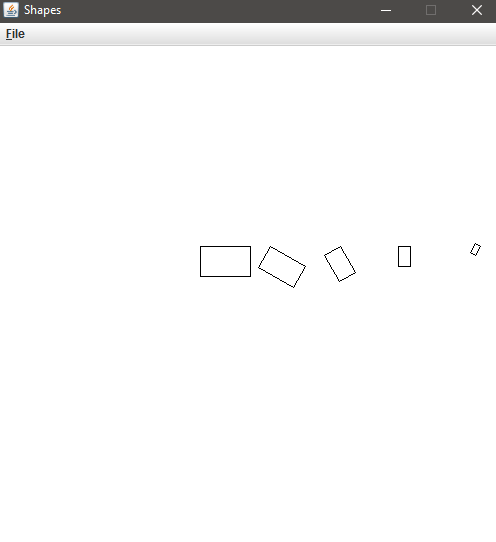
\includegraphics[width=0.7\textwidth, height = 0.3\pdfpageheight, keepaspectratio]{../img/w06-lab/RollingRectangle.png}
\caption {Resultatet av \newline \code{RectangleSequence(Rectangle(Point(200, 200), 50, 30, 0), 5, 0, 70, -30, 0.67)}.}
\label{fig:classes:turtlegraphics:rollingrectangle}
\end{figure}


\begin{figure}[H]
\centering
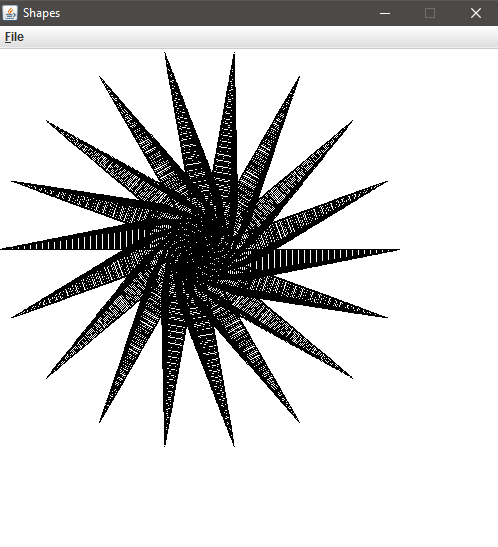
\includegraphics[width=0.7\textwidth, height = 0.3\pdfpageheight,keepaspectratio]{../img/w06-lab/RectangleSequence.png}
\caption {Resultatet av följande kodsnutt.}
\label{fig:classes:turtlegraphics:rectanglesequence}

\end{figure}
\begin{Code}
val w = new SimpleWindow(500, 500, "Shapes")
val t = new Turtle(w, new Point(200, 200), 0, false)
val rect = Rectangle(Point(225, 235), 50, 30, 0)
val roll = RectangleSequence(rect, 100, 0, 2, 0, 0.98)
     
for(i <- 0 to 360 by 20) 
      roll.rotateLeft(i).draw(t)
 
\end{Code}